\documentclass[a4paper,12pt,onepage]{book}
\usepackage[utf8]{inputenc}
\title{}
\author{Rachel Morris}
\date{\today}

\usepackage{rachwidgets}
\usepackage{fancyhdr}
\usepackage{lastpage}
\usepackage{boxedminipage}

\newcommand{\laClass}{CS 250\ }
\newcommand{\laSemester}{Fall 2017\ }

\pagestyle{fancy}
\fancyhf{}
\lhead{\laClass}
\chead{\laSemester}
\rhead{Project 1: Linked Lists}
\rfoot{\thepage\ of \pageref{LastPage}}
\lfoot{By Rachel Morris, \footnotesize last updated \today}

\renewcommand{\headrulewidth}{2pt}
\renewcommand{\footrulewidth}{1pt}

\begin{document}

    \chapter*{Project 1: Linked List} \stepcounter{chapter}
    
        \begin{center}
            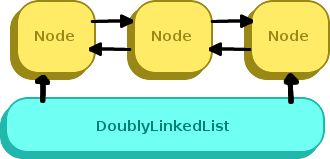
\includegraphics{images/linked-list-title.png}
        \end{center}

        \section*{Information}
            \paragraph{ Topics: } Linked lists, pointers, basic program implementation
            \paragraph{ Turn in: } All source files (.cpp and .hpp).
            \paragraph{ Starter files: } Download on GitHub or D2L.
        
        \subsection*{About}
    
            In this project, you will be implementing a Doubly Linked List.
            
            There are two parts of the project: The tests, and an actual program.
            When you start the program, it will ask you which to run.
            
\begin{lstlisting}[style=output]
-----------------------
1. Run tests
2. Run program
3. Exit
>> 
\end{lstlisting}

            For the first part of the assignment, you will work on implementing
            the DoublyLinkedList, using the tests to verify your work.
            For the second part, you will go into the \texttt{project1\_program}
            and replace usage of the STL \texttt{list} with your DoublyLinkedList
            instead.

\renewcommand*\DTstylecomment{\rmfamily\color{green}\textsc}

\begin{framed}
\dirtree{%
.1 Project 1 - Linked List/.
.2 project1\_main{.}cpp
    \dots{} \begin{minipage}[t]{5cm} Contains main() \end{minipage}.
.2 project1\_LinkedList{.}hpp
    \dots{} \begin{minipage}[t]{5cm} Class declaration \end{minipage}.
.2 project1\_LinkedList{.}cpp
    \dots{} \begin{minipage}[t]{6cm} Class function definitions \end{minipage}.
.2 project1\_Tester{.}hpp
    \dots{} \begin{minipage}[t]{6cm} Unit test functions \end{minipage}.
.2 project1\_{CustomerData.hpp}
    \dots{} \begin{minipage}[t]{6cm} CustomerData, the data stored in the LinkedList \end{minipage}.
.2 project1\_{CustomerData.cpp}.
.2 project1\_{program.hpp}
    \dots{} \begin{minipage}[t]{6cm} The program functionality \end{minipage}.
.2 project1\_{program.cpp}.
.2 cuTEST/
    \dots{} \begin{minipage}[t]{6cm} Unit test framework \end{minipage}.
.3 Menu{.}hpp.
.3 StringUtil{.}hpp.
.3 TesterBase{.}hpp.
.3 TesterBase{.}cpp.
.2 CodeBlocks Project/
    \dots{} \begin{minipage}[t]{6cm}
        Code::Blocks project file
    \end{minipage}.
.3 VS2015 Project 1
    \dots{} \begin{minipage}[t]{6cm}
        Visual Studio project files
    \end{minipage}.
}
\end{framed}

Your project needs to be compiling as a C++11 project. To set this up
in Code::Blocks, go to Settings, Compiler, then in the Compiler Flags
pane, check the ``Have g++ follow the C++11 ISO C++ language standard".

% ----------------------------------------------------------------------
% ----------------------------------------------------------------------
% ----------------------------------------------------------------------
    \newpage
    \section*{Linked List basics}

        A linked list is a type of structure that only allocates memory for new objects as-needed.
        Unlike the Dynamic Array, it doesn't pre-allocate large chunks of memory and resize as 
        needed. Instead, each time a new item is pushed into the list, memory for a new ``Node" 
        is allocated.

        A linked list requires two different classes: A Node and a LinkedList.

    \subsection*{Node}
        
        \begin{wrapfigure}{r}{0.4\textwidth}
        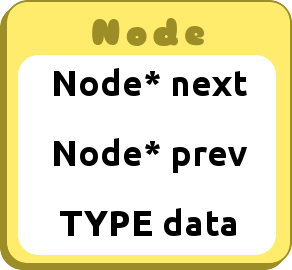
\includegraphics[height=4cm]{images/justanode.png}
        \end{wrapfigure}
    
        A Node contains the data itself, as well as pointers. In a doubly-linked-list, 
        the Node contains pointers to the next node and the previous node.
        In a singly-linked-list, the node only contains a pointer to the next node.

        Using these previous and next pointers to nodes, we can traverse the list by updating 
        a ``traversal" pointer... starting at the first node, and step-by-step going 
        to each node's next pointer.
        
        When a Node is first created, its next and previous pointers should
        be pointing to \texttt{nullptr}.
    
    \subsection*{LinkedList}
        
        \begin{wrapfigure}{r}{0.4\textwidth}
        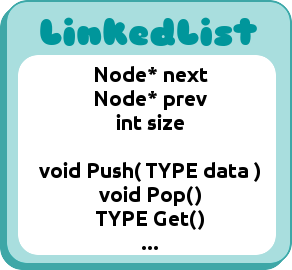
\includegraphics[height=4cm]{images/justalist.png}
        \end{wrapfigure}
        
        The LinkedList class contains the main functionality of the list,
        such as Push to add new items, Pop to remove items, and Get to access items.
        The LinkedList also contains pointers to the first item in the list and,
        often, the last item in the list (though not required).
        The LinkedList is also responsible for keeping track of how many items
        have been added.

        When a LinkedList is empty, whether when it is first created or if everything
        has been removed, the first and last pointers should be ponting to
        \texttt{nullptr}.
        
        When the LinkedList is destroyed, its destructor should be responsible
        for freeing up all the memory allocated for the Node items.

    \subsection*{Adding new items}
    
        When a Push or Insert function is called, the LinkedList needs to...
        
        \begin{itemize}
            \item \textbf{allocate memory for the new Node}
            \item \textbf{update the pointers of any existing Nodes that will be the new Node's neighbor}
            \item \textbf{update the pointer for the first or last item in the LinkedList.}
        \end{itemize}
    
        As we add new items to the linked list, each new element needs memory allocated.
        To do this, create a local pointer variable within the function, then allocate the 
        memory for the Node, and set up the Node's data.
        
\begin{lstlisting}[style=code]
void Push( T data )
{
    Node* newNode = new Node;
    newNode->data = data;
    m_itemCount++;
    // ...
}
\end{lstlisting}
    
        What we do with this newNode will then depend based on whether or not the
        LinkedList is empty, or if it contains at least one item.
        
        \paragraph{Empty LinkedList:}
        
            \begin{center}
                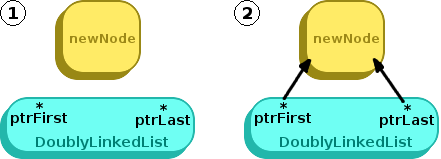
\includegraphics[height=4cm]{images/linkedlist-empty-newnode.png}
            \end{center}
            
            Once a new Node is created, if our LinkedList is empty, the only step
            we have to do is update its \textit{first} and \textit{last} Node* pointers
            to the newNode that we've created.
        
        \newpage
        \paragraph{Non-empty LinkedList:}
        
            \begin{center}
                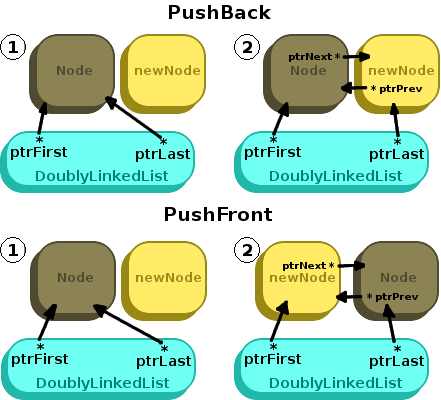
\includegraphics[height=8cm]{images/linkedlist-existing-newnode.png}
            \end{center}
            
            If the LinkedList is \textbf{not} empty, there are more steps
            you will have to take care of. These steps also depend on whether
            you're writing a \textbf{Push Back} (insert as new end) 
            or \textbf{Push Front} (insert as new beginning) function.
            
            \begin{itemize}
                \item PushBack:
                \begin{enumerate}
                    \item Set the current \textit{last Node}'s next pointer to the new node.
                    \item Set the new node's previous pointer to the current \textit{last Node}.
                    \item Update the \textit{last Node} pointer of the LinkedList to point at the new Node.
                \end{enumerate}
                
                \item PushFront:
                \begin{enumerate}
                    \item Set the current \textit{first Node}'s previous pointer to the new node.
                    \item Set the new node's next pointer to the current \textit{first Node}.
                    \item Update the \textit{first Node} pointer of the LinkedList to point at the new Node.
                \end{enumerate}
            \end{itemize}
    
    
        \begin{error}{Don't delete!}
        You won't need to call delete in the same function; the Pop function will be responsible for freeing any allocated memory.    
        \end{error}
        
        
    \subsection*{Removing items}
    
        When you remove an item from the LinkedList, you will have to update
        the pointers of the LinkedList, as well as any Nodes that were neighbors
        to the Node that was removed. Additionally, the two scenarios that
        have different behaviors here are if the LinkedList contains 
        \textit{only one item} (so you're removing the last item), or
        if it contains more than one item.
        
        \paragraph{Pop when list is empty?}
        
            If Pop is called and the list is already empty, the usual
            behavior is to ignore it.
            
            For example, if we were using the STL \texttt{list},
            we can see on its documentation page
            (http://www.cplusplus.com/reference/list/list/pop\_back/) its
            exception safety level:
            
            \begin{center}
                \begin{mdframed}
                    \textbf{Exception safety}
                    If the container is not empty, the function never 
                    throws exceptions (no-throw guarantee).
                    Otherwise, it causes \textit{undefined behavior}.
                \end{mdframed}
            \end{center}
        
        \paragraph{Removing last item}
        
            If you're removing the last item from the LinkedList, you
            will have to make sure to free the memory for the Node,
            but also update the LinkedList's Node pointers to the 
            first and last item; these should both point at \texttt{nullptr}.
            
\begin{lstlisting}[style=code]
void Pop( T data )
{
    // It is the last item
    if ( m_ptrFirst == m_ptrLast )
    {
        delete m_ptrFirst;
        m_ptrFirst = nullptr;
        m_ptrLast = nullptr;
        m_itemCount--;
    }
    // ...
}
\end{lstlisting}
        
        \newpage
        \paragraph{Pop when we have more than one item in the list}
        
            In our DoublyLinkedList we can Pop items off from the front
            of the list or the back of the list, so the way to
            implement this changes a bit for each.
        
            \begin{center}
                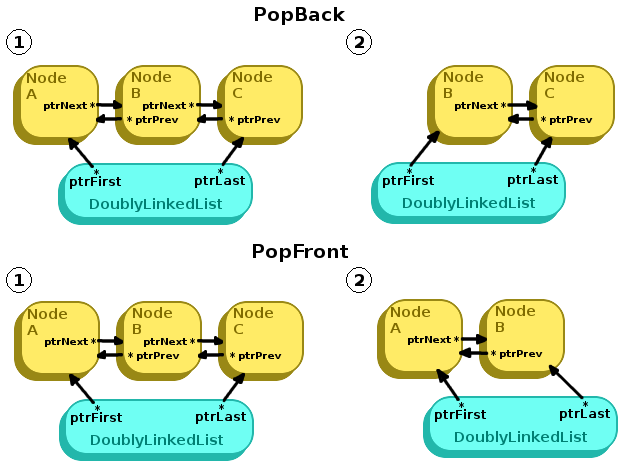
\includegraphics[height=9cm]{images/linkedlist-popping.png}
            \end{center}
    
            \begin{itemize}
                \item PopBack:
                \begin{enumerate}
                    \item Locate the second-to-last item in the LinkedList (With a DoublyLinkedList, you can
                        simply get the last Node's \textit{previous} item.)
                    \item Update the second-to-last Node's next pointer to be \texttt{nullptr}.
                    \item Free the memory pointed to by the last Node pointer
                    \item Update the last Node pointer to point to the (formerly) second-to-last Node
                    \item Decrease the item count
                \end{enumerate}
                
                \item PopFront:
                \begin{enumerate}
                    \item Locate the second item in the LinkedList (You can
                        get the first Node's \textit{next} item.)
                    \item Update the second Node's previous pointer to be \texttt{nullptr}.
                    \item Free the memory pointed to by the first Node pointer
                    \item Update the first Node pointer to point to the (formerly) second Node
                    \item Decrease the item count
                \end{enumerate}
            \end{itemize}
            
            \begin{hint}{Keeping track of the second Node}
                Your code might look ugly if you're trying to do these steps like
\begin{verbatim}
m_ptrLast->ptrPrev->ptrNext = nullptr;
\end{verbatim}
                
                Instead of working like this, simply make a local Pointer
                to keep track of your second-to-last or second item...
                
\begin{verbatim}
// PopBack
Node* ptrSecondToLast = m_ptrLast->m_ptrPrev;
ptrSecondToLast->ptrNext = nullptr;
// ...

// PopFront
Node* ptrSecond = m_ptrFirst->m_ptrNext;
ptrSecond->ptrPrev = nullptr;
// ...
\end{verbatim}                
            \end{hint}
    
    \subsection*{List traversal}

        When traversing the list, we need to make a traversal pointer, 
        which begins at the first item, and steps through each node via 
        each node's ptrNext pointer.

        We cannot randomly access data in a linked list because it is not 
        implemented with an array. Because we only keep track of the first 
        and last item with pointers, we have to traverse the list to find some 
        item at position n.

        First, we create a pointer:

    \begin{verbatim} 
        Node<T>* ptrCurrent;
    \end{verbatim} 

        We do not allocate memory with this pointer! This pointer is meant to point at existing data.

        To begin at the beginning of the list, you need to point this to the first item:

    \begin{verbatim} 
        ptrCurrent = m_ptrFirst;
    \end{verbatim} 

        And to step to the next item, make use of ptrNext:

    \begin{verbatim} 
        ptrCurrent = ptrCurrent->ptrNext; // Go to the next item
    \end{verbatim} 
        
        If you want to go to item n in the list, then you'll just have to do the above step n times (via a loop.)

        You can traverse a few ways. If you have a specific position you want to stop at, use an integer counter.

        If you want to traverse over a full list, you can loop while the traversal pointer is not nullptr.
        
    \section*{Common errors}
    
        \subsection*{New node pointer vs. Traversal pointer}
    
        It is common to mix up utilizing pointers for list traversal with utilizing pointers for making new nodes. Know whether you're traversing a list, or creating a new node!

        When traversing, \underline{you will not allocate new memory!}

    \chapter*{Doubly Linked List specs}

\end{document}









